\documentclass[a4paper,10pt]{article}

\usepackage[english]{babel}
\usepackage[utf8]{inputenc}
\usepackage{graphicx}
\usepackage{amsmath}
\usepackage{amssymb}
\usepackage{amsbsy}
\usepackage{eucal}
\usepackage{hyperref, url}
\usepackage{float}
\usepackage{verbatim} % For verbatiminput.
\usepackage{fancyvrb}
\usepackage{afterpage}
\usepackage{program}

\pdfinfo{            
          /Title      (T-61.3050 Machine Learning: Basic Principles)
          /Author     ()
          /Keywords   ()
}

\DefineVerbatimEnvironment {code}{Verbatim}
   {%numbers=left,numbersep=2mm,
     %frame=lines,framerule=0.1mm, 
     fontsize=\small}
\RecustomVerbatimCommand{\VerbatimInput}{VerbatimInput}
   {%numbers=left,numbersep=2mm,
     frame=lines,framerule=0.1mm, fontsize=\small}
\DefineVerbatimEnvironment {outputlog}{Verbatim}
  {frame=lines,framerule=0.1mm, fontsize=\small}

\newcommand{\XXX}[1]{{\bf XXX #1}}
\parindent 0mm
\parskip 3mm

%------------------------------------------------------------------------------
% First page
%------------------------------------------------------------------------------

% add your student number in parenthesis
\title{T-61.3050 Term Project, final report\\ % Dictated in instructions.
       Using decision trees for spam classification}
\author{Jori Bomanson (81819F) \\
  {\tt jori.bomanson@aalto.fi} \\
  \\
  Sami J. Lehtinen (44814P)\\ 
  {\tt sjl@iki.fi} \\
}
\begin{document}

\floatstyle{plain}
\newfloat{Listing}{t}{lol}
\floatname{Listing}{Listing}

\maketitle
\thispagestyle{empty}
\pagebreak
\pagenumbering{arabic}

\section{Abstract}
% Include the key points of your work in a few sentences (including methods
% used and conclusions).
We programmed and trained a univariate binary classification tree to detect
spam email. We studied the importance of different training set sizes,
10-fold cross validation as well as prepruning and postpruning techniques.

\XXX{summary of conclusions and their importance}


\section{Rationale}

The choice of using a decision tree to solve a task with boolean variables
seemed natural. Such a tree could definitely match whatever complexity there
would be in the training data.
In fact we figured our success would be determined mainly by how we would
manage to avoid overfitting.

Decision trees were also tempting in that they are much easier to
visualize than, e.g., naive bayes classifiers.  For example, see
figure \ref{fig:prune-both-pruned-6000}.

One reason to study decision trees was that we assumed many groups would
take on naive bayesian classifiers, and we wanted to do something a bit
different.

When we started the project, we actually didn't realize that we could
use existing libraries for the job.  This led us to implement a decision
tree algorithm by hand instead of just taking, e.g., an existing
$C5.0$\cite{c50} implementation.

\section{Principles of decision trees}

Decision trees are a non-parametric method for data classification.
They don't try to approximate any model behind the data, instead relying
on a tactic of ``similar inputs produce similar outputs''.

Our algorithm basically implements the classification tree construction
algorithm in \cite[p. 179]{alpaydin2004}.  There is one change, however.
We thought it would be a good idea to use the split entropy when
checking for minimum entropy.  The pseudocode is listed in figure
\ref{fig:tree-gen}.

\begin{figure}[th]
  \centering
  \begin{minipage}[c]{1.0\textwidth}
\begin{program}
  \PROC |generate_tree|(|data|) \BODY
  |impurity| \leftarrow |MAX|
  \FOR i:= 1 \TO |num_columns| \DO
       |im| \leftarrow |calculate_impurity|(|data|, |column|)
       \IF |im| < |impurity| 
       \THEN
          |impurity| \leftarrow |im|
          |split_column| \leftarrow i
       \FI
       \OD
  \IF |impurity| < \theta 
  \THEN
       |create_leaf_node|(column, |label|)
       \rcomment { |label| will be the majority class in the |data|. }
       \EXIT 
       \FI
  X_{tagged}, X_{untagged} \leftarrow |split|(|data|, |column|)
  \COMMENT{Generate both child nodes by splitting with the chosen\
    attribute, i.e., column.}
  |generate_tree|(X_{tagged})
  |generate_tree|(X_{untagged})
  \ENDPROC
  \PROC |calculate_impurity|(|data|, |column|) \BODY
  X_{tagged}, X_{untagged} \leftarrow |split|(|data|, |column|)
  |impurity|(X_{tagged}, X_{untagged})
  \rcomment{Impurity is calculated using equation \ref{eqn:impurity}.}
  \ENDPROC
\end{program}
  \end{minipage}
  \caption{Pseudo-code for tree generation algorithm.}
  \label{fig:tree-gen}
\end{figure}

\subsection{Calculating impurity}

We chose to measure impurity with the entropy function
\cite[p. 176]{alpaydin2004}\footnote{Alpaydin cites ``(Quinlan 1986)''
  for the impurity algorithm.}.

\begin{equation}
\begin{split}
\mathcal{I}'_m &= - \sum_{j=1}^n\frac{N_{mj}}{N_m}\sum_{i=1}^K p_{mj}^i 
    \log p_{mj}^i  \label{eqn:impurity} \\
\text{for a node} \quad & m  \\
\text{where} \quad 0 \log 0 &\equiv 0  \\
p_m^i &= P(\text{Instance reaching node m belongs to class i})  \\
K &= 2
\end{split}
\end{equation}

\subsection{Pruning the tree}

Decision trees can be trained to perfectly match the training
data\cite[p. 182]{alpaydin2004}.  This will lead the model to
gross overfitting, which manifests as a large generalization error.
This can be avoided by pruning the tree.  There are two non-exclusive
approaches to pruning, prepruning and postpruning.

Without pruning, a tree with a training set size of 1000 looks like
figure \ref{fig:no-pruning-1000}.

\begin{figure}[h]
  \centering
  \begin{minipage}[c]{1.0\textwidth}
    \centering
\includegraphics[width=130mm]{postpruned-original-1000.pdf}
  \end{minipage}
  \caption{Tree from training set of 1000 elements, that hasn't been
    pruned.}
  \label{fig:no-pruning-1000}
\end{figure}

Still, against the test set the non-pruned tree faired surprisingly
well, achieving an accuracy of over 94 percent.

Trees with various training set sizes and prunings are depicted in
figures \ref{fig:prepruned-1000}, \ref{fig:prune-both-original-6000},
\ref{fig:prune-both-pruned-6000}, and \ref{fig:no-pruning-6000}.

\subsubsection{Prepruning}

In prepruning, the recursion of the training algorithm is stopped once
certain limits are reached.  Examples include impurity and number of
data rows.

In our first versions of the classifier we only did prepruning, which
resulted in very small and tidy trees, but the accuracy left comething
to be desired (94-95 percent).  We used one of the suggested
approaches from \cite{alpaydin2004}, where we make the tree as pure as
possible (no prepruning) and handle overfitting by postpruning the tree.

Removing prepruning didn't have an adverse effect for the final
accuracy, indeed, accuracy increased by a couple percentage points with
a large training set (6000). {\XXX new results!}

\begin{figure}
  \centering
\begin{tabular}{|l|l|r|c|c|c|c|}
\hline
Size & Pruning & Training time & Accuracy & Precision & Recall &
Perplexity \\ \hline 
1000 & post & 38 & 0.953 & 0.984 & 0.944 & 1.215 \\
1000 & both & 38 & 0.944 & 0.985 & 0.930 & 1.165 \\
2000 & post & 118 & 0.961 & 0.984 & 0.956 & 1.194 \\
2000 & both & 113 & 0.966 & 0.983 & 0.965 & 1.175 \\
4000 & post & 381 & 0.971 & 0.982 & 0.973 & 1.141 \\
4000 & both & 380 & 0.970 & 0.985 & 0.970 & 1.136 \\
6000 & post & 683 & 0.971 & 0.985 & 0.971 & 1.128 \\
6000 & both & 668 & 0.977 & 0.991 & 0.974 & 1.138 \\
8000 & post & 1112 & 0.977 & 0.988 & 0.978 & 1.111 \\
8000 & both & 1033 & 0.971 & 0.982 & 0.975 & 1.117 \\
\hline
\end{tabular}
  \caption{Effects of pruning on accuracy and other characteristics with
    various training data sizes.}
  \label{tbl:classifiers} 
\end{figure}

We implemented prepruning by having three different stopping criteria in
our algorithm to limit the depth of the resulting tree.  The first ensures
that there's always atleast one feature to base a decision on, the second
that there's enough messages and the third that there's enough entropy to
warrant further recursion.  For example, \XXX{more detailed explanation}.

1000 items in training set, theta = 0.04, min\_row\_ratio = 0.002

\begin{figure}[h]
  \centering
  \begin{minipage}[c]{1.0\textwidth}
    \centering
\includegraphics[width=130mm]{prune-both-original-1000.pdf}
  \end{minipage}
  \caption{Prepruned tree from a training set of 1000 elements.}
  \label{fig:prepruned-1000}
\end{figure}

\subsubsection{Postpruning}
\label{sect:postpruning}

Postpruning is used to reduce generalization error by using a special
pruning data set to check whether removing a subtree from the decision
tree will result in the same or smaller error against the pruning set.
The complexity of such a subtree is deemed unjustified and we expect
to avoid overfitting by substituting them with simple leaf nodes,
labeled according to the majority class of the training instances
reaching them\cite[p. 183]{alpaydin2004}.

\begin{figure}[h]
  \centering
  \begin{minipage}[c]{1.0\textwidth}
    \centering

\includegraphics[width=130mm]{prune-both-original-6000.pdf}
  \end{minipage}
  \caption{Prepruned tree from a training set of 6000 elements.}
  \label{fig:prune-both-original-6000}
\end{figure}

\begin{figure}[h]
  \centering
  \begin{minipage}[c]{1.0\textwidth}
    \centering

\includegraphics[width=130mm]{prune-both-pruned-6000.pdf}
  \end{minipage}
  \caption{Pre- and postpruned tree from a training set of 6000 elements.}
  \label{fig:prune-both-pruned-6000}
\end{figure}

\XXX{table of errors with a postpruned tree}
\begin{figure}[h]
  \centering
  \begin{minipage}[c]{1.0\textwidth}
    \centering
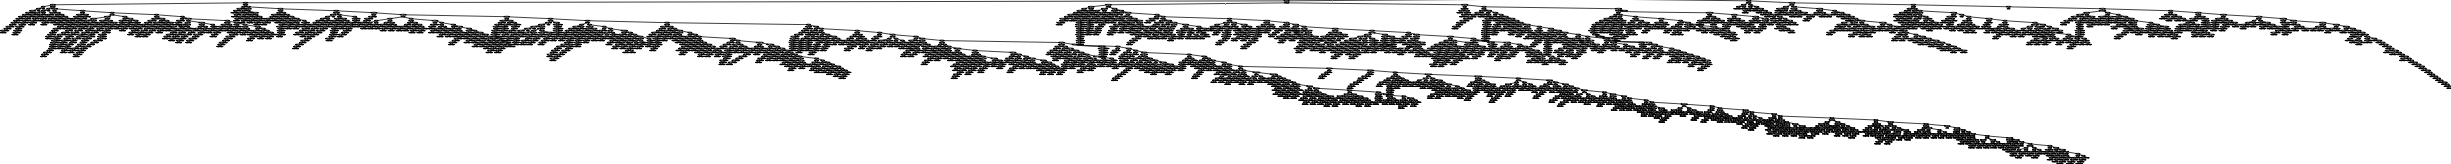
\includegraphics[width=130mm]{postpruned-pruned-6000.pdf}
  \end{minipage}
  \caption{Postpruned tree from a training set of 6000 elements.}
  \label{fig:no-pruning-6000}
\end{figure}

It should be noted that training the set without prepruning takes
slightly longer than with it.

Prepruned tree takes a small hit in accuracy, but is slightly faster to
train, both according to our observations and
Alpaydin\cite[p. 182]{alpaydin2004}.

\section{Validation of our approach}

\subsection{Accuracy, precision, recall, and perplexity}

The criteria for measuring the goodness of the classifier are the same
as the ones used in the data challenge.  As described in
\cite{termproject}, accuracy is the fraction of test set messages
classified correctly.  The precision is the ratio of correctly
classified spam messages to all messages classified as spam.  Recall is
the ratio of correctly classified spam messages to all spam messages.

Perplexity is calculated with

\begin{equation}
P = \exp(-\operatorname{mean}(\ln{Pi}))
\end{equation}

where $Pi$ is the probability of the email message being of the correct
class.

For the perplexity calculation, we return the probability that a message
is spam based on the ratio of spam messages left at the leaf node that
ends up deciding whether the message is spam or not.  This seems a
decent metric for calculating perplexity, at least when comparing to
what other groups reported in the data challenge.

\subsection{K-fold cross validation}

We implemented 10-fold cross validation to our classifier.  This
gave more stable values for generalization error when compared to
repeatedly training the classifier without the cross validation.

One part of the training data set was used for postpruning the tree, see
section \ref{sect:postpruning}.

\subsection{Dummy model}


\section{Results with different training set sizes}


\subsection{Training algorithm complexity}

Based on figure \ref{tbl:classifiers}, training algorithm looks like a
$O(n\log{n})$ algorithm.  Definitely not quadratic, although not linear,
either.

\section{Data challenge}

% what did we do based on the results of the data challenge.

The data challenge led us to realize that our - at the time merely
prepruned - decision tree wasn't the magical black box method
that would wipe the table that we hoped it would be.
As a consequence we did the inevitable and gave postpruning,
as well K-fold cross validation a try.


\section{Conclusions}

The chosen approach didn't achieve the same high marks for accuracy as
the winners of the data challenge.  Tweaking of the approach is
naturally possible, but it seems that decision trees are more suited in
this as a part of combined classifier instead of on their own.  This
does not mean that the approach is completely without merits; decision
trees were applied here without prior knowledge to the distribution of
the spam messages.  In the data challenge, the winning teams had tweaked
the prior probabilities for spam to match the distribution in the data
set.  In the decision tree model, this is not necessary, or even
possible.

Looking at the generated decision trees, it is easy to follow the
process by eye (at least with the smaller trees).  This, we think, helps
a lot in validating the approach.

We implemented the algorithm with Python and Numpy ourselves.  We think
this gave us deeper insight into the inner workings of the algorithm
than just using an existing software package.

From the final results, we see (figure \ref{tbl:classifiers}) that we
get the best accuracy 97.7\% with 6000 data points.

It would've been interesting to see how
boosting\cite[p. 360]{alpaydin2004} would've affected the results;
unfortunately, we didn't have time to try it.  Because our classifier
was already producing quite good results, boosting might have given that
extra percentage point or so.

\section{Comments on project difficulty}

Writing the classifier by hand took quite a bit of effort.  Even though
the algorithm is simple in principle, testing it was perceived hard to
automate.  As a result, testing was done ad-hoc by the developer, taking
time off writing features (such as boosting).

We underestimated the difficulty of the task, which became apparent when
the results of the data challenge were published.

The project was challenging, but not too much so.

\begin{figure}
  \centering
\begin{tabular}{|l|c|c|}
\hline
 & Classifier & Report \\ \hline
Sami & 32h & 8+h \\ % from git logs and calendar.
Jori & 20h & 5h  \\ % mutuilua
\hline
\end{tabular}
  \caption{Estimated hours for the project}
  \label{tbl:effort-estimate} 
\end{figure}

%\afterpage{\clearpage} % Flush all floats so that they won't mingle with
%                       % the python code, below.
\pagebreak
\begin{thebibliography}{9}
\bibitem{alpaydin2004}
  Ethem Alpaydin,
  \emph{Introduction to Machine Learning}.
  Massachusetts Institute of Technology, Cambridge, Massachusetts,
  1st edition,
  2004. 415 pages. ISBN 0-262-01211-1.
\bibitem{termproject}
  \emph{Term Project 2011: Spam or Ham?}.
  \href{https://noppa.aalto.fi/noppa/kurssi/t-61.3050/term\_project}
  {https://noppa.aalto.fi/noppa/kurssi/t-61.3050/term\_project}
  [Web article]. 2011-11-6. [Cited 2011-11-19].
\bibitem{c50}
  \emph{Data Mining Tools See5 and C5.0}.
  \href{http://rulequest.com/see5-info.html}
  {http://rulequest.com/see5-info.html}
  [Web article]. 2011-01. [Cited 2011-11-20].

%\bibitem{press07}
%  William H. Press, Saul A. Teukolsky, William T. Vetterling, Brian P. Flannery,
%  \emph{Numerical recipes - the art of scientific computing}.
%  Cambridge University Press, New York,
%  3rd edition,
%  2007. 1235 pages. ISBN 978-0-521-88068-8.
%\bibitem{mellin10a}
%  Ilkka Mellin, 
%  \emph{Todennäköisyyslaskenta ja tilastotiede: Kaavat}.
%  Otaniemi, 2010. 390 pages.
%\bibitem{mellin10b}
%  Ilkka Mellin, 
%  \emph{Tilastolliset taulukot}.
%  Otaniemi, 2010. 13 pages.
\end{thebibliography}

\appendix
\section{Python code for the classifier}

The code is available for scrutiny at GitHub,
\href{https://github.com/sjlehtin/spam-or-ham/blob/master/decisiontree.py}
{https://github.com/sjlehtin/spam-or-ham/blob/master/decisiontree.py}.

% From the term project page:
% 
% Please, do not hand in any programs or source code you may have
% written. They will not be graded. (You should naturally include
% pseudocode etc. to your report if it helps to understand what you have
% done. Be sure to refer to pseudocode etc. in the text.)
%\verbatiminput{decisiontree.py}

\end{document}
